\section{Hierarchical Navigable Small World (HNSW)}

\subsection{Introduction to HNSW}

Hierarchical Navigable Small World (HNSW) is a graph-based approach for approximate nearest neighbor (ANN) search, built on navigable small-world (NSW) networks with a controllable hierarchical structure. It was initially introduced by Malkov and Yashunin as an arXiv preprint in 2016 \cite{Malkov-Yashunin-2016} and later published in the peer-reviewed \textit{IEEE Transactions on Pattern Analysis and Machine Intelligence} in 2020 \cite{Malkov-Yashunin-2020}.

HNSW incrementally builds a multi-layered structure composed of hierarchical proximity graphs, where each layer corresponds to a nested subset of the stored elements. The maximum layer in which an element appears is selected randomly according to an exponentially decaying probability distribution \cite{Malkov-Yashunin-2016}.

Starting the search from the upper layer, together with utilizing scale separation, boosts performance compared to NSW and allows logarithmic complexity scaling \cite{Malkov-Yashunin-2016}. Performance evaluations have shown that HNSW remains one of the state-of-the-art approaches for vector search \cite{erikbern-ann-benchmarks}, leading to its adoption in various vector databases and search systems.

The HNSW implementation is available at GitHub\footnote{\url{https://github.com/nmslib/hnswlib}}.

\subsection{Building Blocks of HNSW}

\subsubsection{Navigable Small World (NSW)}

Navigable Small World (NSW), predecessor of HNSW, is a graph-based approach for approximate nearest neighbor (ANN) search. It combines two key ideas: short-range connections that approximate the Delaunay triangulation, and long-range connections that ensure the small-world navigation property (Figure~\ref{fig:hnsw-1} \cite{Malkov-Ponomarenko-Logvinov-Krylov-2014}). The short-range edges preserve local proximity information required for greedy search, while long-range edges maintain overall graph connectivity and enable polylogarithmic scalability of search complexity. A distinctive feature of the NSW construction is that long-range links arise naturally: as new elements are inserted consecutively and connected to their nearest neighbors, some of the previously added edges gradually become long-range connections \cite{Malkov-Ponomarenko-Logvinov-Krylov-2014}.

An important limitation of NSW lies in its routing process, which can be divided into two phases: "zoom-out" and "zoom-in" \cite{Malkov-Yashunin-2016}. In the "zoom-out" phase, the search expands outward from a low-degree node, progressively reaching high-degree nodes (hubs), while in the "zoom-in" phase the routing converges towards the target through increasingly local, short-range connections \cite{Boguna-Krioukov-Claffy-2007}. Starting the search directly from hubs, thereby skipping the "zoom-out" stage, reduces the probability of getting stuck in a distant false local minimum and improves efficiency. Nevertheless, the overall routing in NSW still exhibits only polylogarithmic complexity. This shortcoming motivated the introduction of a hierarchical structure in HNSW to achieve logarithmic search complexity \cite{Malkov-Yashunin-2016}.

\begin{figure}[H]
    \centering
    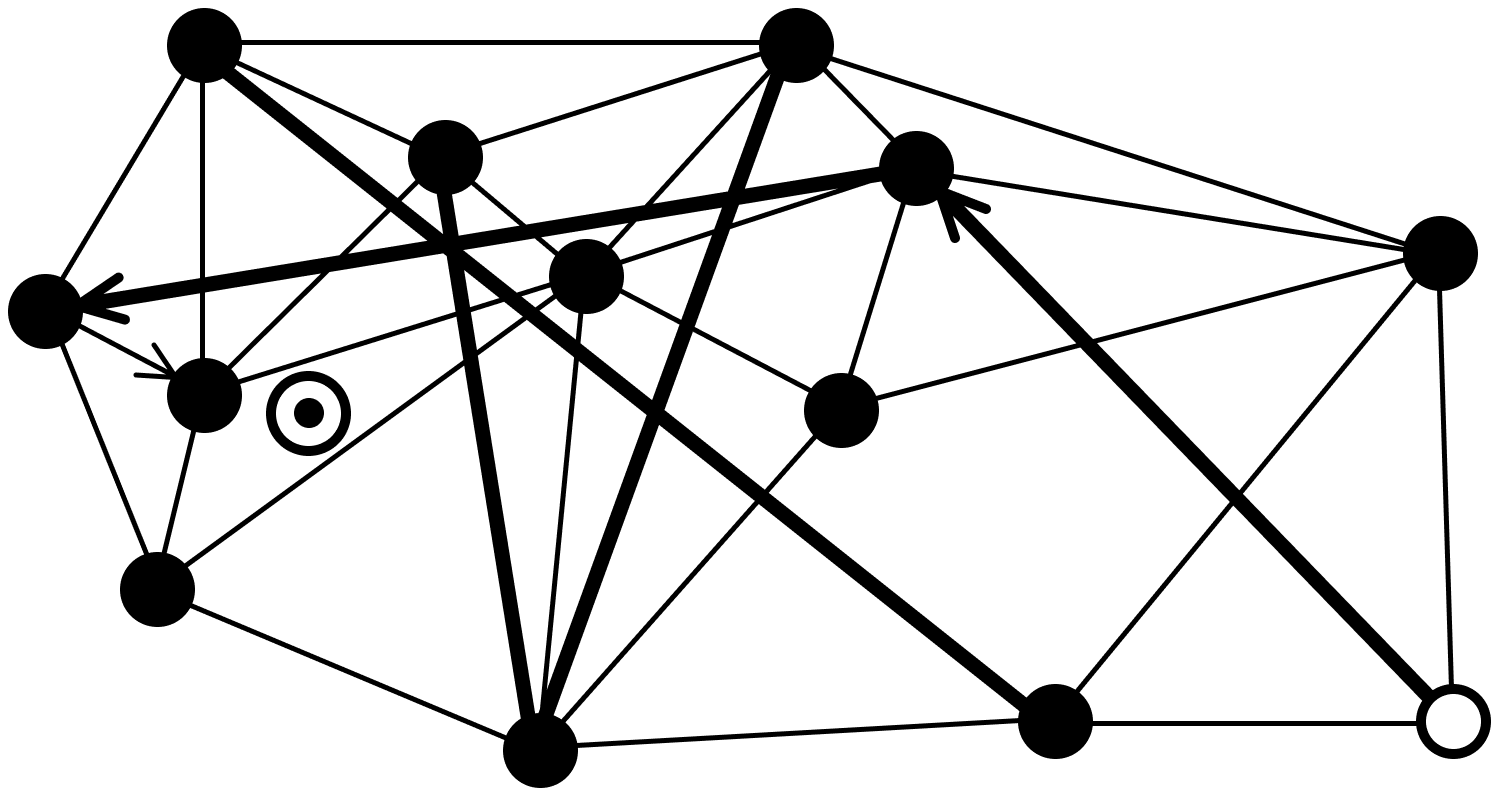
\includegraphics[width=0.6\textwidth]{chapters/algorithms/hnsw/figures/nsw.png}
    \caption{Graph representation of an NSW structure. Filled circles represent data points, while the entry point and the query point are indicated as an empty circle and a target circle, respectively. Thin edges represent short-range connections preserving local proximity, and thick edges represent long-range connections ensuring overall graph connectivity and enabling polylogarithmic search complexity. Arrows illustrate the path of the greedy search from the entry point to the query.}
    \label{fig:hnsw-1}
\end{figure}

\paragraph{The Small World Problem}

Social psychologist Milgram investigated \cite{Milgram-1967} how individuals are connected into social networks through ties of kinship and acquaintance, and whether short paths exist between any two randomly chosen people. To test this, he devised an experimental method: participants were given the name and basic information of a target person. If they did not personally know the target, they were instructed to forward the folder to a personal acquaintance who was more likely to know the target, restricted to contacts they knew on a first-name basis.

The experiment revealed that the median number of intermediaries required to connect two individuals was approximately 5.5, providing empirical evidence for the small-world phenomenon (popularly known as \textit{six degrees of separation} \cite{Guare-1990}).

\subparagraph{Navigability}

Computer scientist Kleinberg studied \cite{Kleinberg-2000-5, Kleinberg-2000-8} how individuals can efficiently find short paths in large social networks using only local information. He modeled networks following the small-world paradigm, characterized by dense short-range connections and a few random long-range links. While small-world networks guarantee that short paths exist between any two nodes, this does not ensure that a decentralized algorithm can discover them.

Kleinberg showed that there exists a unique value of a parameter controlling the distribution of long-range links at which a greedy algorithm can navigate efficiently, with expected delivery time scaling polylogarithmically with $N$, where $N$ is the number of nodes. For other values of this parameter, navigation becomes asymptotically inefficient. These results indicate that navigability is not a general property of all small-world networks but only emerges under specific structural conditions.

\paragraph{Proximity Graph}

Proximity graphs are geometric graphs in which two vertices $p$ and $q$ are connected by an edge $(p, q)$ if and only if a certain exclusion region defined for $p$ and $q$ contains no other points from the vertex set. Depending on the choice of the exclusion region, various types of proximity graphs can be defined, such as the Delaunay triangulation \cite{Mitchell-Mulzer-2017}.

\newpage

\subparagraph{Voronoi Diagram}

Given a set of points in the plane (Figure~\ref{fig:hnsw-2-a} \cite{Moghaddam-Banihashemi-Bakhshoodeh-Mir-Delgado-2023}), a Voronoi diagram partitions the plane according to the nearest-neighbor rule: each point is associated with the region of the plane that is closest to it (Figure~\ref{fig:hnsw-2-b} \cite{Moghaddam-Banihashemi-Bakhshoodeh-Mir-Delgado-2023}). Voronoi diagrams naturally arise in various proximity problems, such as the classical post-office problem, which asks how a fixed set of points can be preprocessed to quickly determine the nearest point to an arbitrary query location, and its generalization to finding the $k$ nearest points \cite{Aurenhammer-1991}.

\begin{figure}[H]
    \centering
    \begin{subfigure}[t]{0.48\textwidth}
        \centering
        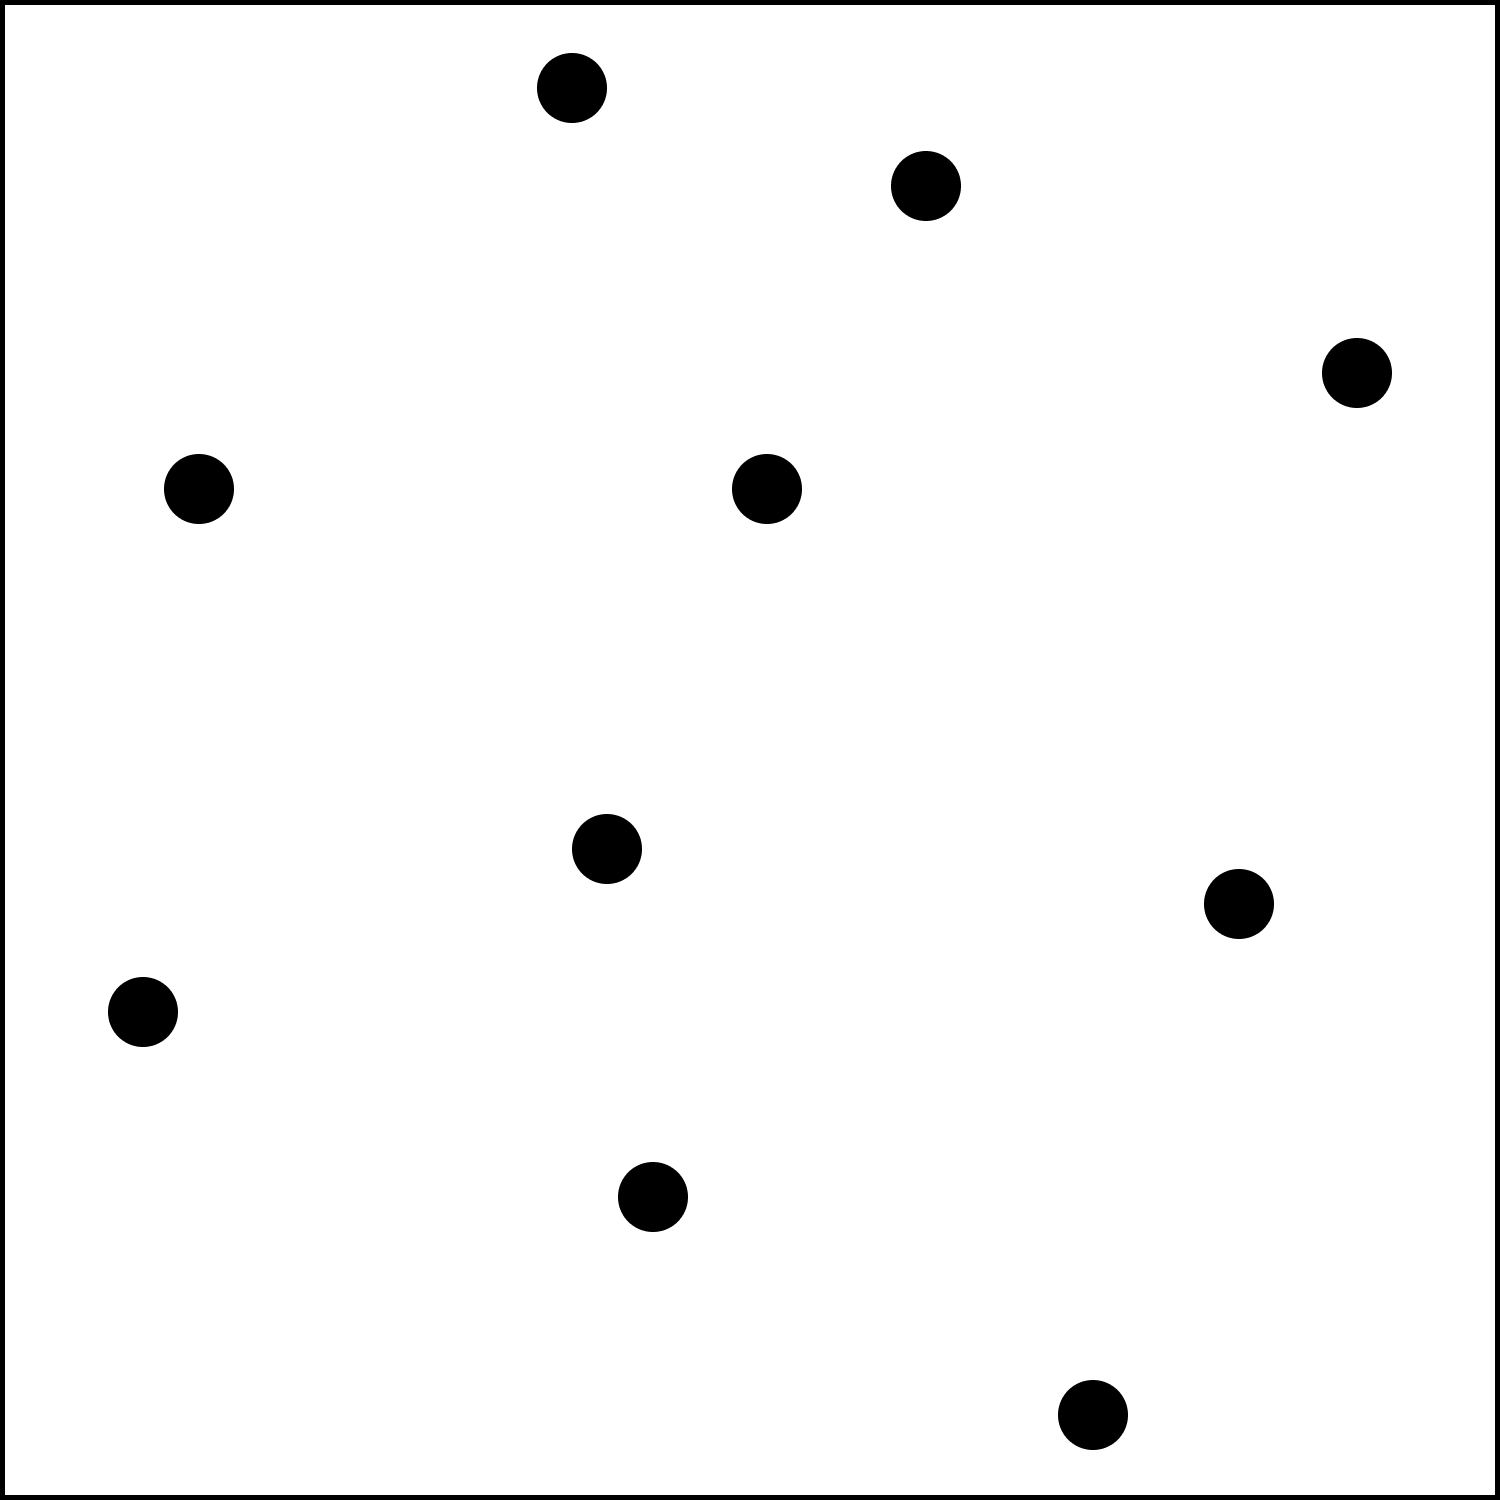
\includegraphics[width=\textwidth]{chapters/algorithms/hnsw/figures/voronoi-points.png}
        \caption{Data points in the plane.}
        \label{fig:hnsw-2-a}
    \end{subfigure}
    \hfill
    \begin{subfigure}[t]{0.48\textwidth}
        \centering
        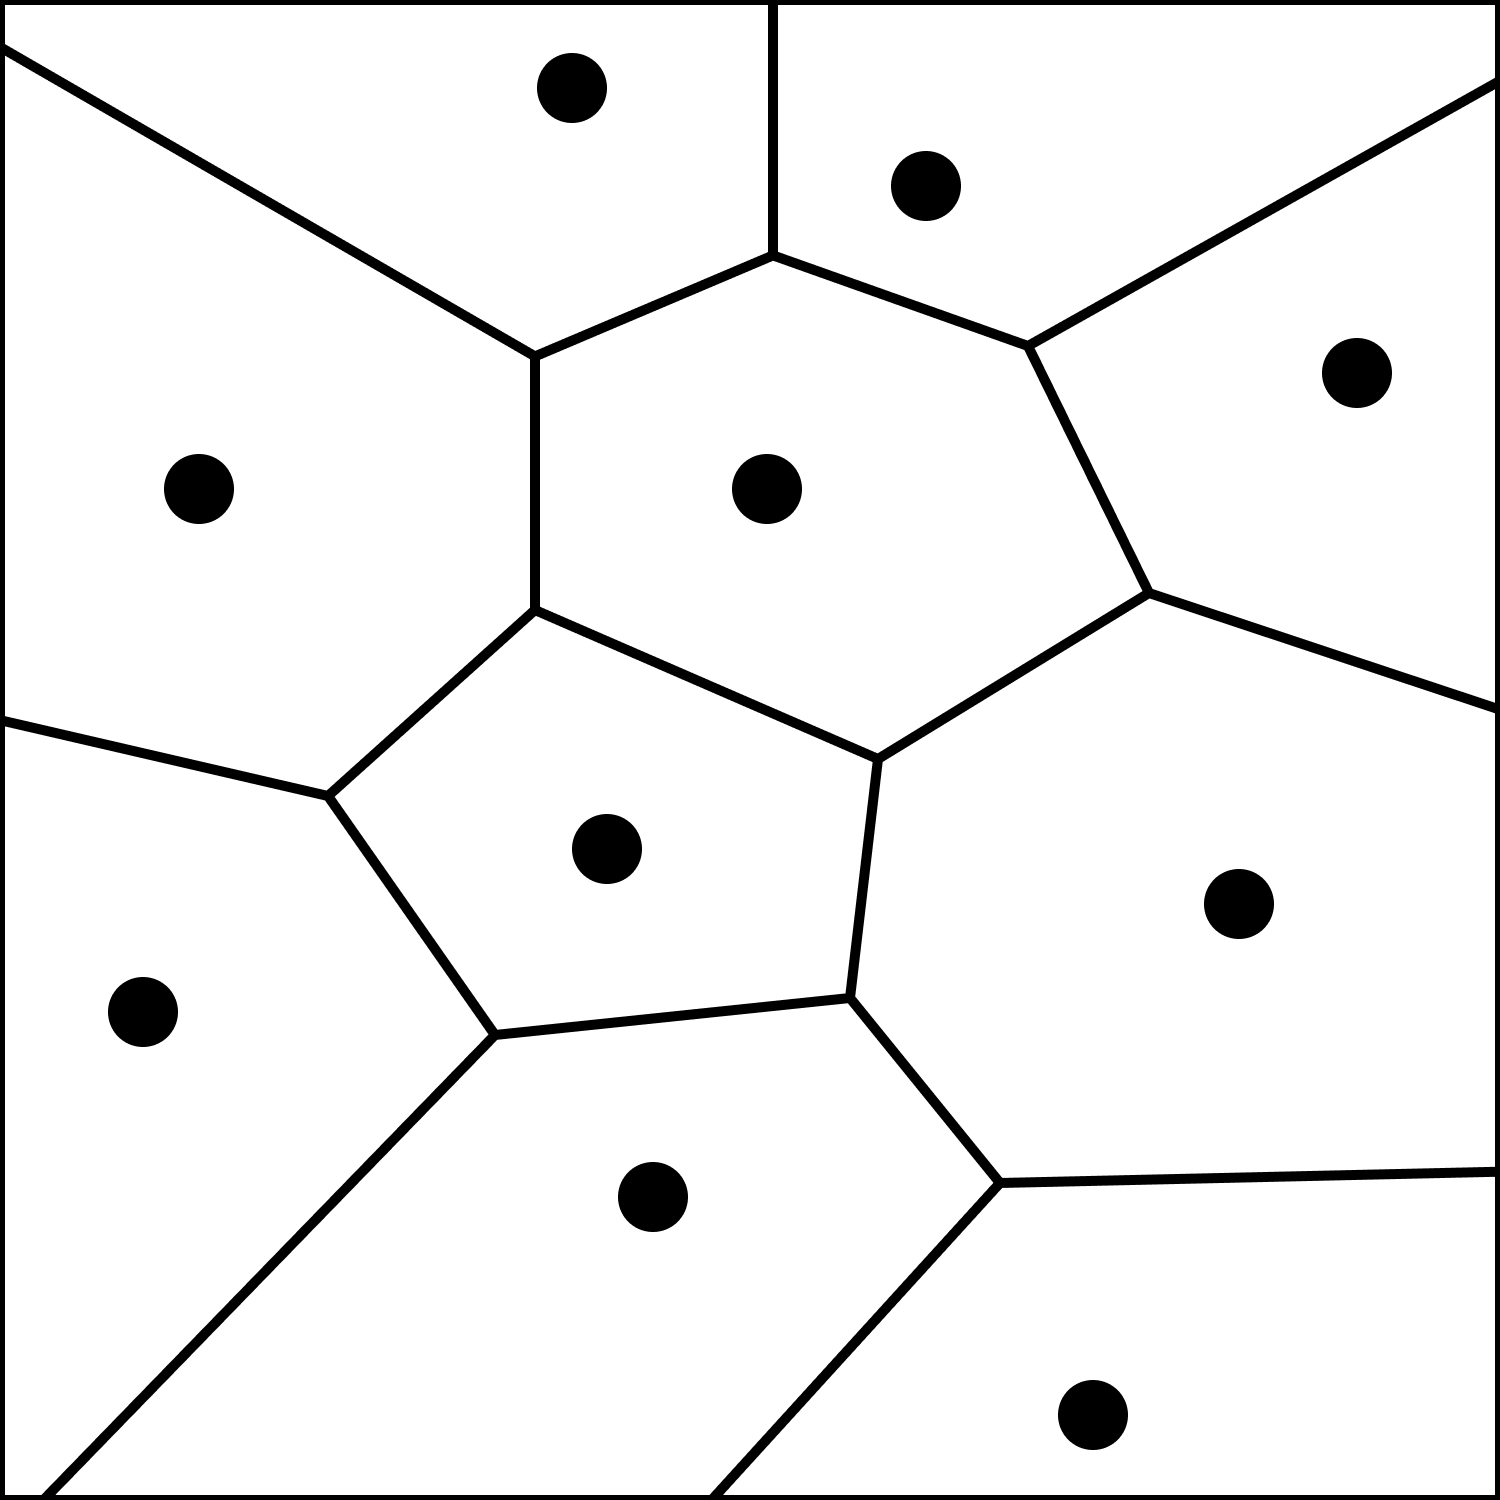
\includegraphics[width=\textwidth]{chapters/algorithms/hnsw/figures/voronoi-diagram.png}
        \caption{Voronoi diagram of the points, showing nearest-neighbor regions.}
        \label{fig:hnsw-2-b}
    \end{subfigure}
    \caption{Voronoi diagram illustration: (a) data points, (b) nearest-neighbor partitioning of the plane.}
    \label{fig:hnsw-2}
\end{figure}

\subparagraph{Delaunay Triangulation}

Delaunay triangulation is closely related to Voronoi diagrams: two points are connected by a straight-line edge if and only if their Voronoi regions share a boundary (Figure~\ref{fig:hnsw-3} \cite{Moghaddam-Banihashemi-Bakhshoodeh-Mir-Delgado-2023}). It can also be defined using the empty-circle property, where triangles are formed such that the circumcircle of each triangle contains no other point, and the set of these edges constitutes the triangulation.

As the geometric dual of the Voronoi diagram, Delaunay triangulation preserves local proximity information by linking neighboring points \cite{Aurenhammer-1991}. A key property of the Delaunay graph is that greedy search is guaranteed to find the true nearest neighbor \cite{Malkov-Yashunin-2016}.

Despite this advantage, constructing the Delaunay graph requires prior knowledge of the metric space \cite{Navarro-2002} and suffers from the curse of dimensionality \cite{Aurenhammer-1991}. Moreover, since exactness is not required in approximate nearest neighbor search, maintaining the full Delaunay graph is unnecessary \cite{Malkov-Ponomarenko-Logvinov-Krylov-2014}.

\begin{figure}[H]
    \centering
    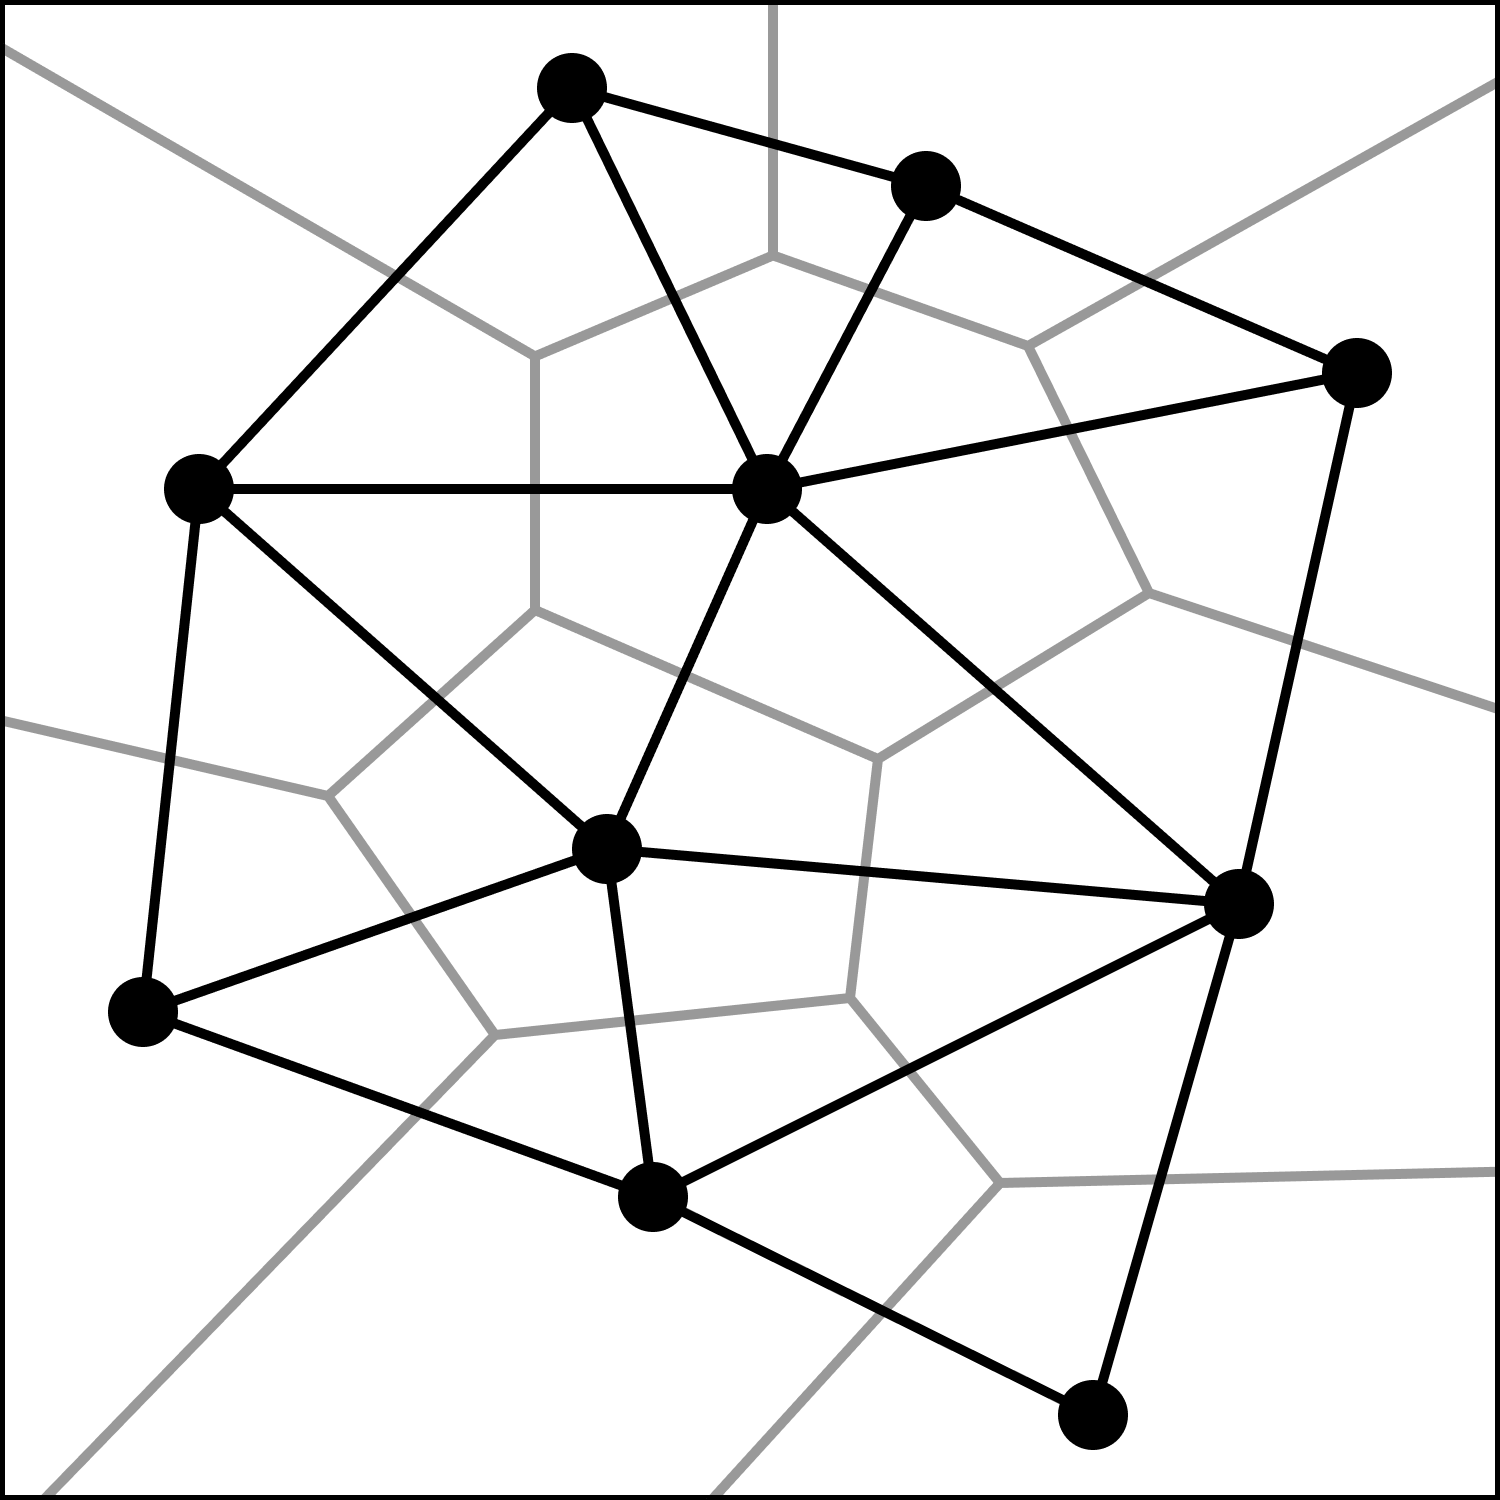
\includegraphics[width=0.48\textwidth]{chapters/algorithms/hnsw/figures/delaunay.png}
    \caption{Delaunay triangulation constructed on top of the Voronoi diagram, connecting points whose Voronoi regions share a boundary.}
    \label{fig:hnsw-3}
\end{figure}

\subsubsection{Skip List}

HNSW can alternatively be interpreted as an extension of the probabilistic skip list structure, where the linked lists are replaced by proximity graphs \cite{Malkov-Yashunin-2016}. This perspective highlights the hierarchical organization of elements across multiple layers, similar to how skip lists allow efficient search through multiple levels of linked nodes.

\subsection{Description of HNSW}

The algorithm organizes elements into multiple layers: upper layers contain longer links and fewer elements, while lower layers contain shorter links and more elements. This design enables efficient search by starting from the upper layer (the "zoom-in" phase), greedily moving toward a local minimum, and then descending to lower layers, restarting from the local minimum found in the previous layer (Figure~\ref{fig:hnsw-4} \cite{Malkov-Yashunin-2016}).

Unlike NSW, elements do not need to be shuffled before insertion. Instead, stochasticity is introduced through level randomization, which supports truly incremental indexing even under temporary changes in data distribution \cite{Malkov-Yashunin-2016}.

\begin{figure}[H]
    \centering
    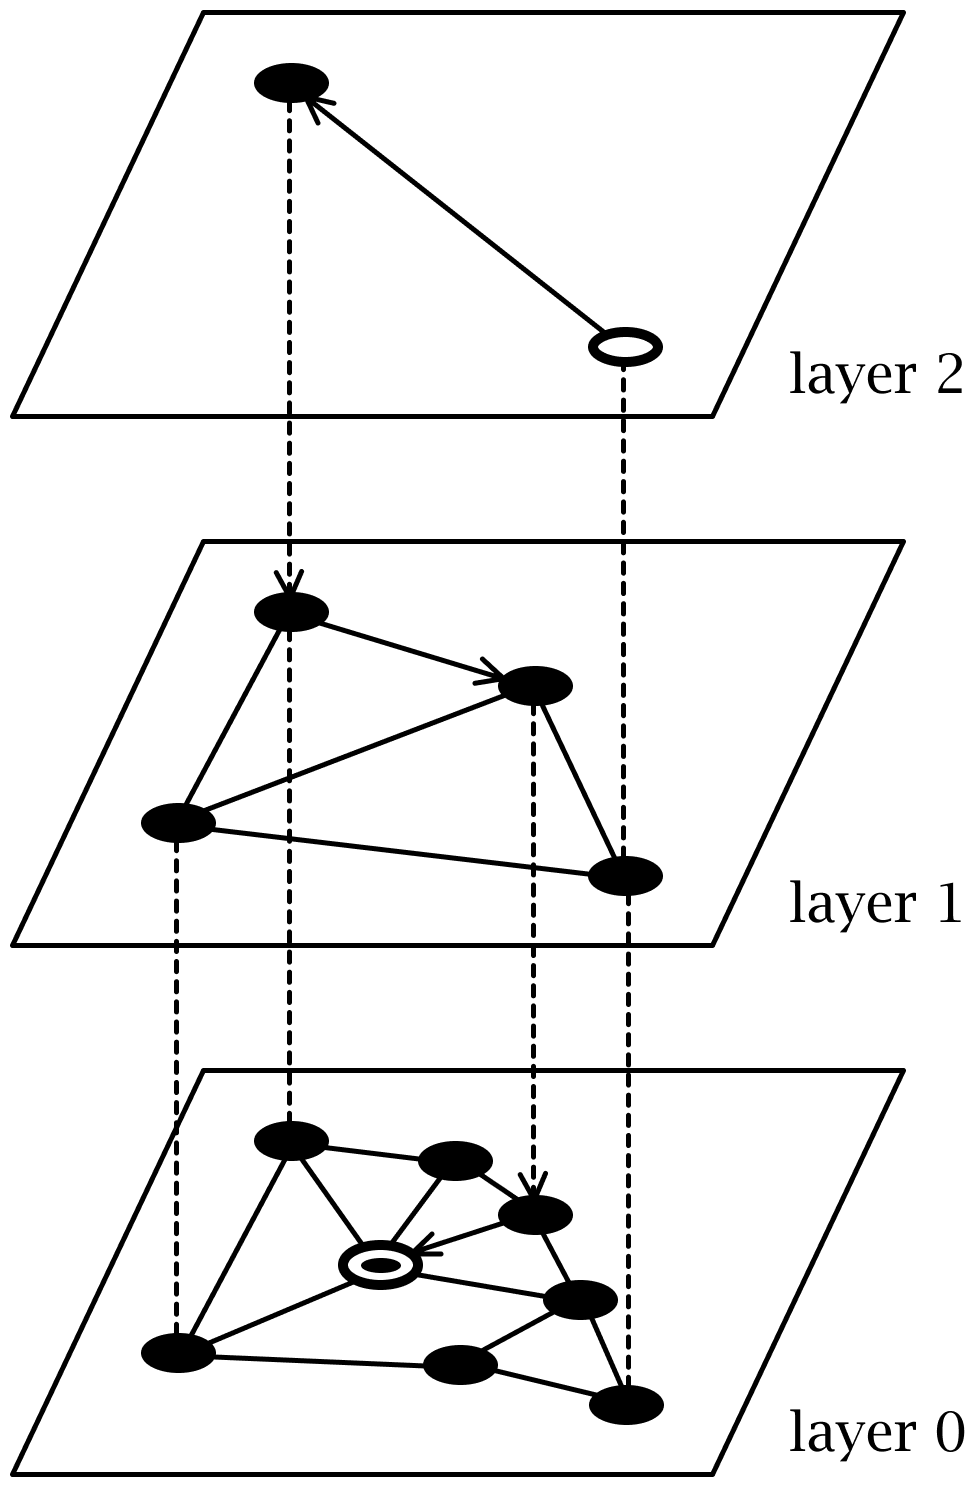
\includegraphics[width=0.4\textwidth]{chapters/algorithms/hnsw/figures/hnsw.png}
    \caption{Graph representation of an HNSW structure. Filled circles represent data points, while the entry point and the query point are indicated as an empty circle and a target circle, respectively. Arrows illustrate the path of the greedy search across layers, starting from the upper layer and descending to lower layers. Upper layers contain longer links and fewer elements, while lower layers contain shorter links and more elements.}
    \label{fig:hnsw-4}
\end{figure}

\paragraph{Element Insertion}

The construction of the HNSW structure is based on consecutive insertions of new elements into the multilayer graph (Algorithm~\ref{alg:hnsw-1}). For each element $q$, a maximum layer $l$ is sampled from a geometric distribution controlled by the parameter $m_L$.

The insertion begins at the top layer $L$, where the algorithm performs a greedy search to find the $ef$ closest neighbors of $q$. The search then proceeds layer by layer down to level $l + 1$, each time using the best candidates from the previous layer as entry points. At layers $l$ down to $0$, the algorithm performs a broader greedy search to identify the $efConstruction$ closest neighbors of $q$, from which up to $M$ are selected to establish bidirectional connections. If the degree of a neighboring element exceeds $M_{\text{max}}$ (or $M_{\text{max0}}$ at the ground layer), its connections are pruned using the same neighbor selection procedure.

Finally, if $q$ is assigned a level higher than the current maximum, it becomes the new entry point of the structure \cite{Malkov-Yashunin-2016}.

\begin{algorithm}[H]
    \caption{INSERT \cite{Malkov-Yashunin-2016}}
    \label{alg:hnsw-1}
    \begin{algorithmic}[1]
        \Require multilayer graph $hnsw$, new element $q$, number of established connections $M$, maximum number of connections per element per layer $M_{\text{max}}$, size of dynamic candidate list $efConstruction$, normalization factor for level generation $m_L$
        \Ensure updated $hnsw$ with element $q$ inserted
        
        \State $W \gets \emptyset$ \Comment{list of currently found nearest elements}
        \State $ep \gets$ get entry point of $hnsw$
        \State $L \gets$ level of $ep$ \Comment{top layer in $hnsw$}
        \State $l \gets \lfloor -\ln(\text{$unif$}(0..1)) \cdot m_L \rfloor$ \Comment{level of new element}
        
        \For{$l_c \gets L \dots l+1$} 
            \State $W \gets \text{SEARCH-LAYER}(q, ep, ef=1, l_c)$
            \State $ep \gets$ get nearest element from $W$ to $q$
        \EndFor
        
        \For{$l_c \gets \min(L,l) \dots 0$} 
            \State $W \gets \text{SEARCH-LAYER}(q, ep, efConstruction, l_c)$
            \State $neighbors \gets \text{SELECT-NEIGHBORS}(q, W, M, l_c)$ \Comment{Algorithm~\ref{alg:hnsw-3} or~\ref{alg:hnsw-4}}
            \State add bidirectional connections from $neighbors$ to $q$ at layer $l_c$
            
            \For{each $e \in neighbors$} \Comment{shrink connections if necessary}
                \State $eConn \gets$ $neighborhood(e)$ at layer $l_c$
                \If{$|eConn| > M_{\text{max}}$} \Comment{shrink connections of $e$ (if $l_c = 0$, then $M_{\text{max}} = M_{\text{max0}}$)}
                    \State $eNewConn \gets \text{SELECT-NEIGHBORS}(e, eConn, M_{\text{max}}, l_c)$ \Comment{Algorithm~\ref{alg:hnsw-3} or~\ref{alg:hnsw-4}}
                    \State set $neighborhood(e)$ at layer $l_c$ to $eNewConn$
                \EndIf
            \EndFor
            
            \State $ep \gets W$
        \EndFor
        
        \If{$l > L$}
            \State set entry point of $hnsw$ to $q$
        \EndIf
    \end{algorithmic}
\end{algorithm}

\paragraph{ANN Layer Search}

To obtain the approximate $ef$ nearest neighbors of a query element $q$ within a given layer $l_c$, the algorithm (Algorithm~\ref{alg:hnsw-2}) maintains a list $W$ of up to $ef$ closest found elements, initialized with the entry points. At each step, the closest non-evaluated element from the candidate set $C$ is selected, and its neighbors are examined. If a neighbor is closer to $q$ than the furthest element currently in $W$, or if $W$ contains fewer than $ef$ elements, it is added to both $C$ and $W$. The process continues until all elements in $C$ have been evaluated.

A key stopping condition is that once the closest candidate in $C$ is further from $q$ than the most distant element in $W$, the search terminates, as no remaining candidates can improve the result. This mechanism prevents unnecessary distance evaluations and avoids bloating of the search structures \cite{Malkov-Yashunin-2016}.

\begin{algorithm}[H]
    \caption{SEARCH-LAYER \cite{Malkov-Yashunin-2016}}
    \label{alg:hnsw-2}
    \begin{algorithmic}[1]
        \Require query element $q$, entry points $ep$, number of nearest neighbors $ef$, layer number $l_c$
        \Ensure $ef$ nearest neighbors to $q$
        
        \State $v \gets ep$ \Comment{set of visited elements}
        \State $C \gets ep$ \Comment{set of candidates}
        \State $W \gets ep$ \Comment{dynamic list of found nearest neighbors}
        
        \While{$|C| > 0$}
            \State $c \gets$ extract nearest element from $C$ to $q$
            \State $f \gets$ get furthest neighbor from $W$ to $q$
            \If{$distance(c, q) > distance(f, q)$}
                \State \textbf{break} \Comment{all elements in $W$ evaluated}
            \EndIf
            
            \For{each $e \in$ $neighborhood(c)$ at layer $l_c$} \Comment{update $C$ and $W$}
                \If{$e \notin v$}
                    \State $v \gets v \cup \{e\}$
                    \State $f \gets$ get furthest neighbor from $W$ to $q$
                    \If{$distance(e, q) < distance(f, q)$ \textbf{or} $|W| < ef$}
                        \State $C \gets C \cup \{e\}$
                        \State $W \gets W \cup \{e\}$
                        \If{$|W| > ef$}
                            \State remove furthest neighbor from $W$ to $q$
                        \EndIf
                    \EndIf
                \EndIf
            \EndFor
        \EndWhile
        
        \State \Return $W$
    \end{algorithmic}
\end{algorithm}

\paragraph{Simple Neighbor Selection}

A straightforward approach for selecting connections in the proximity graph is to simply select the closest elements to the base element from the candidate set (Algorithm~\ref{alg:hnsw-3}). This strategy does not account for the mutual distances between candidates, but only their distances to the base element, which may lead to redundant connections in highly clustered regions of the space \cite{Malkov-Yashunin-2016}.

\begin{algorithm}[H]
    \caption{SELECT-NEIGHBORS-SIMPLE \cite{Malkov-Yashunin-2016}}
    \label{alg:hnsw-3}
    \begin{algorithmic}[1]
        \Require base element $q$, candidate elements $C$, number of neighbors to return $M$
        \Ensure $M$ nearest elements to $q$
        
        \State \Return $M$ nearest elements from $C$ to $q$
    \end{algorithmic}
\end{algorithm}

\paragraph{Heuristic Neighbor Selection}

To address the limitations of the simple strategy, a heuristic procedure is employed for selecting neighbors (Algorithm~\ref{alg:hnsw-4}). The heuristic processes the candidates in order of increasing distance to the base element and establishes a connection to a candidate only if its distance to the base element is smaller than its distance to any of the already selected neighbors. In this way, the algorithm promotes diversity of connections by preventing redundant edges in similar directions.
\newpage
Two optional parameters further refine this method. The first, \textit{extendCandidates}, allows the candidate set to be expanded by including neighbors of the initial candidates; although disabled by default, this option is beneficial in extremely clustered data. The second, \textit{keepPrunedConnections}, enables adding back some of the discarded candidates in order to maintain a fixed number of connections per element \cite{Malkov-Yashunin-2016}.

\begin{algorithm}[H]
    \caption{SELECT-NEIGHBORS-HEURISTIC \cite{Malkov-Yashunin-2016}}
    \label{alg:hnsw-4}
    \begin{algorithmic}[1]
        \Require base element $q$, candidate elements $C$, number of neighbors to return $M$, layer number $l_c$, flag indicating whether or not to extend candidate list $extendCandidates$, flag indicating whether or not to add discarded elements $keepPrunedConnections$
        \Ensure $M$ elements selected by the heuristic

        \State $R \gets \emptyset$
        \State $W \gets C$ \Comment{queue for candidates}

        \If{$extendCandidates$} \Comment{extend candidates by their neighbors}
            \For{each $e \in C$}
                \For{each $e_{adj} \in$ $neighborhood(e)$ at layer $l_c$}
                    \If{$e_{adj} \notin W$}
                        \State $W \gets W \cup \{e_{adj}\}$
                    \EndIf
                \EndFor
            \EndFor
        \EndIf

        \State $W_d \gets \emptyset$ \Comment{queue for discarded candidates}

        \While{$|W| > 0$ \textbf{and} $|R| < M$}
            \State $e \gets$ extract nearest element from $W$ to $q$
            \If{$e$ is closer to $q$ compared to any element from $R$}
                \State $R \gets R \cup \{e\}$
            \Else
                \State $W_d \gets W_d \cup \{e\}$
            \EndIf
        \EndWhile

        \If{$keepPrunedConnections$} \Comment{add some of discarded connections from $W_d$}
            \While{$|W_d| > 0$ \textbf{and} $|R| < M$}
                \State $R \gets R \cup \{$extract nearest element from $W_d$ to $q\}$
            \EndWhile
        \EndIf

        \State \Return $R$
    \end{algorithmic}
\end{algorithm}

\paragraph{$k$-ANN Search}

The retrieval of the $k$ approximate nearest neighbors of a query element $q$ in the HNSW structure (Algorithm~\ref{alg:hnsw-5}) follows a process analogous to inserting a zero-level element. The key distinction is that the closest neighbors at the ground layer are returned as the search result rather than being used to form new connections.

Starting from the top layer $L$, the algorithm traverses down through the layers in a greedy manner. At each layer, the search begins from the element closest to the query found in the previous layer and uses $ef = 1$ to quickly move toward the query. Upon reaching the ground layer ($l_c = 0$), a broader greedy search is conducted with the parameter $ef$ to identify the closest elements, from which the $k$ nearest neighbors are returned \cite{Malkov-Yashunin-2016}.

\begin{algorithm}[H]
    \caption{K-NN-SEARCH \cite{Malkov-Yashunin-2016}}
    \label{alg:hnsw-5}
    \begin{algorithmic}[1]
        \Require multilayer graph $hnsw$, query element $q$, number of nearest neighbors $k$, size of dynamic candidate list $ef$
        \Ensure $k$ nearest neighbors to $q$
        
        \State $W \gets \emptyset$ \Comment{set of current nearest elements}
        \State $ep \gets$ get entry point of $hnsw$
        \State $L \gets$ level of $ep$ \Comment{top layer in $hnsw$}
        
        \For{$l_c \gets L \dots 1$}
            \State $W \gets \text{SEARCH-LAYER}(q, ep, ef=1, l_c)$
            \State $ep \gets$ get nearest element from $W$ to $q$
        \EndFor
        
        \State $W \gets \text{SEARCH-LAYER}(q, ep, ef, l_c=0)$
        \State \Return $k$ nearest elements from $W$ to $q$
        
    \end{algorithmic}
\end{algorithm}

\subsection{Analysis of HNSW}

\subsubsection{Construction Parameters}

The main construction parameters of HNSW are $m_L$, $M_{\text{max0}}$, $M$, and $efConstruction$. These parameters directly influence the graph structure, search performance, and memory usage. The analysis follows \cite{Malkov-Yashunin-2016}.

\paragraph{$m_L$ Parameter}

The parameter $m_L$ controls the probability of assigning elements to higher layers, thereby affecting the hierarchy depth and the navigability of the graph. Its influence can be summarized as: 

\begin{itemize}
    \item $m_L = 0$ and $M_{\text{max0}} = M$: produces a directed $k$-NN graph with power-law complexity.
    \item $m_L = 0$ and $M_{\text{max0}} = \infty$: produces an NSW graph with polylogarithmic complexity.
    \item $m_L > 0$: produces a controllable hierarchy graph with logarithmic complexity.
\end{itemize}

To achieve optimal performance in the controllable hierarchy, the overlap of neighbors across layers (i.e., the percentage of element neighbors shared between layers) should remain small. Reducing $m_L$ decreases this overlap but increases the average number of hops during greedy search, so an optimal tradeoff exists. A practical choice is
\[
m_L = \frac{1}{\ln(M)},
\]
ensuring on average a single overlapping neighbor between layers.

\paragraph{$M_{\text{max0}}$ Parameter}

The parameter $M_{\text{max0}}$ defines the maximum number of connections per element in the ground layer and has a strong influence on search performance, particularly for high-recall queries. Setting $M_{\text{max0}} = M$ leads to a significant performance penalty at high recall. Simulations in \cite{Malkov-Yashunin-2016} suggest that setting $M_{\text{max0}} = 2 \cdot M$ provides good performance, while increasing it further may result in performance degradation and unnecessary memory usage.

\paragraph{$M$ Parameter}

The parameter $M$ defines the number of neighbors to be selected for each element during insertion. It determines how many bidirectional connections a new element establishes in each layer. A reasonable range for $M$ is 5 to 48. Smaller values generally yield better performance for low-dimensional data or low-recall queries, while larger values are more suitable for high-dimensional data or high-recall searches. Memory usage grows proportionally with $M$, so it should be chosen carefully.

\paragraph{$efConstruction$ Parameter}

The parameter $efConstruction$ defines the size of the candidate list used during the insertion of a new element. A sufficiently large $efConstruction$ ensures that most true nearest neighbors of the element are considered, achieving high recall during index construction. Increasing $efConstruction$ can further improve index quality, but at the cost of longer construction times.

\subsubsection{Complexity}

\paragraph{Search Complexity}

A theoretical analysis of a single search, following \cite{Malkov-Yashunin-2016}, assumes exact Delaunay graphs. Suppose the search has identified the closest element at some layer and then descends to the next one. Since the layers are not correlated with the spatial positions of the data points, there is a fixed probability that the next visited node belongs to the upper layer, given by $p = e^{-m_L}$. However, the search within a layer must terminate before reaching such a node; otherwise, the search on the upper layer would have already stopped at a different element. Consequently, the probability of not reaching the target within $s$ steps is bounded by $e^{-s \cdot m_L}$, and the expected number of steps in a layer is given by the geometric series
\[
S = \frac{1}{1 - e^{-m_L}},
\]
which is independent of $N$. If the average degree of a node in the (exact) Delaunay graph is bounded by a constant $C$, then the expected number of distance evaluations per layer is bounded by a constant $C \cdot S$. Since the expected number of layers in the structure grows as $O(\log N)$ by construction, the overall expected search complexity is
\[
O(\log N).
\]

In practice, the assumption of having an exact Delaunay graph is violated in HNSW due to the use of an approximate neighbor selection heuristic with a fixed number of connections per element. To avoid getting stuck in local minima at the ground layer, the greedy search algorithm employs a backtracking procedure. For low-dimensional data, the dependence of the required $ef$ parameter (which controls the number of hops explored during backtracking) on dataset size saturates as $N$ increases, so the backtracking complexity behaves as an additive term and does not affect the overall $O(\log N)$ search scaling \cite{Malkov-Yashunin-2016}.

\paragraph{Construction Complexity}

The index is built by inserting all elements iteratively \cite{Malkov-Yashunin-2016}. Each insertion consists of a sequence of $k$-ANN searches across the layers, followed by applying a heuristic with fixed cost for a given $efConstruction$. The average number of layers an element belongs to is a constant depending only on $m_L$. Therefore, the insertion complexity has the same scaling as the search, and for relatively low-dimensional datasets the overall construction complexity is
\[
O(N \cdot \log N).
\]

\paragraph{Memory Cost}

The memory consumption of HNSW index is primarily determined by the storage of graph connections. Each element has up to $M_{\text{max0}}$ connections in the ground layer and up to $M_{\text{max}}$ connections in all other layers. Therefore, the average memory required per element is 
\[
(M_{\text{max0}} + m_L \cdot M_{\text{max}}) \cdot \text{bytes\_per\_link}.
\]
If the maximum number of elements is limited to approximately four billion, four-byte unsigned integers can be used to store the connections. Typical near-optimal values of $M$ range from 6 to 48, leading to average memory requirements of roughly 60–450 bytes per element, excluding the size of the data itself \cite{Malkov-Yashunin-2016}.